\NewScheme{\SPOR}{SPORES}

\subsection{Message Passing through Predictive Onion Routes (PORs)}
\label{sec:message_passing}


\NewAlgorithm{\Fwd}{Forward}
\NewAlgorithm{\Send}{BuildRouteS}
\NewAlgorithm{\Recv}{BuildRouteR}
\NewAlgorithm{\ExtendRoute}{ExtendRoute}
\NewAlgorithm{\CreateOnionLayer}{CreateLayer}
\NewAlgorithm{\Dec}{Dec}
\NewAlgorithm{\Store}{Store}
\NewVariable{\sk}{sk}
\NewVariable{\rdv}{rdv}
\NewVariable{\LRV}{\mathcal{L_{RV}}\xspace}
\NewVariable{\Hsend}{\mathcal{H}_{\text{send}}\xspace}
\NewVariable{\Hrec}{\mathcal{H}_{\text{rec}}\xspace}
\NewVariable{\Hforward}{\mathcal{H}_f\xspace}
\NewVariable{\Hbackward}{\mathcal{H}_b\xspace}
\NewVariable{\Hsendforward}{\mathcal{H}_{\text{send f}}\xspace}
\NewVariable{\Hsendbackward}{\mathcal{H}_{\text{send b}}\xspace}
\NewVariable{\Hrecforward}{\mathcal{H}_{\text{rec f}}\xspace}
\NewVariable{\Hrecbackward}{\mathcal{H}_{\text{rec b}}\xspace}
\NewVariable{\datakey}{k_{\text{data}}\xspace}
%\NewVariable{\nfilechunks}{\#\text{chunks}}

\david{the use of DeBE algorithms must be explicitly explained in this section}


The principle of onion routing à la Tor~\cite{Tor} is to put nodes relaying messages between a source and a destination.
By employing encryption layers, a relay doesn't know where it is situated on the message's path. 
It only knows who gave him the message, and where to send it to.


In contrast to Tor~\cite{Tor} that provides only one address per hop
in the route, \name provides, for each layer of the onion, several
alternative nodes for the next hop in the route depending on their
probability of being online. 
We call our modified onion routes Probabilistic Onion Routes or PORs.

Another difference from Tor, where connections are established by all nodes in the route, \name is stateless: the route's ends (the sender Alice and receiver Bob) cooperate to create the headers containing all the necessary routing information for future communication between Alice and Bob.
In that regard, two headers are required: \Hforward to route packets from Alice to Bob, and \Hbackward for packets from Bob to Alice.

To implement our predictive onion routing mechanism, \name is thus split in two algorithms: the route building one, and the message routing one.
Figure~\ref{fig:file-exchange} shows the process of the route creation until the first exchange of a file chunk from Alice to Bob.
Alice uses the forward route to send file chunks to Bob, while Bob uses the backward route to send acknowledgments back to Alice.

\begin{figure}[t]
  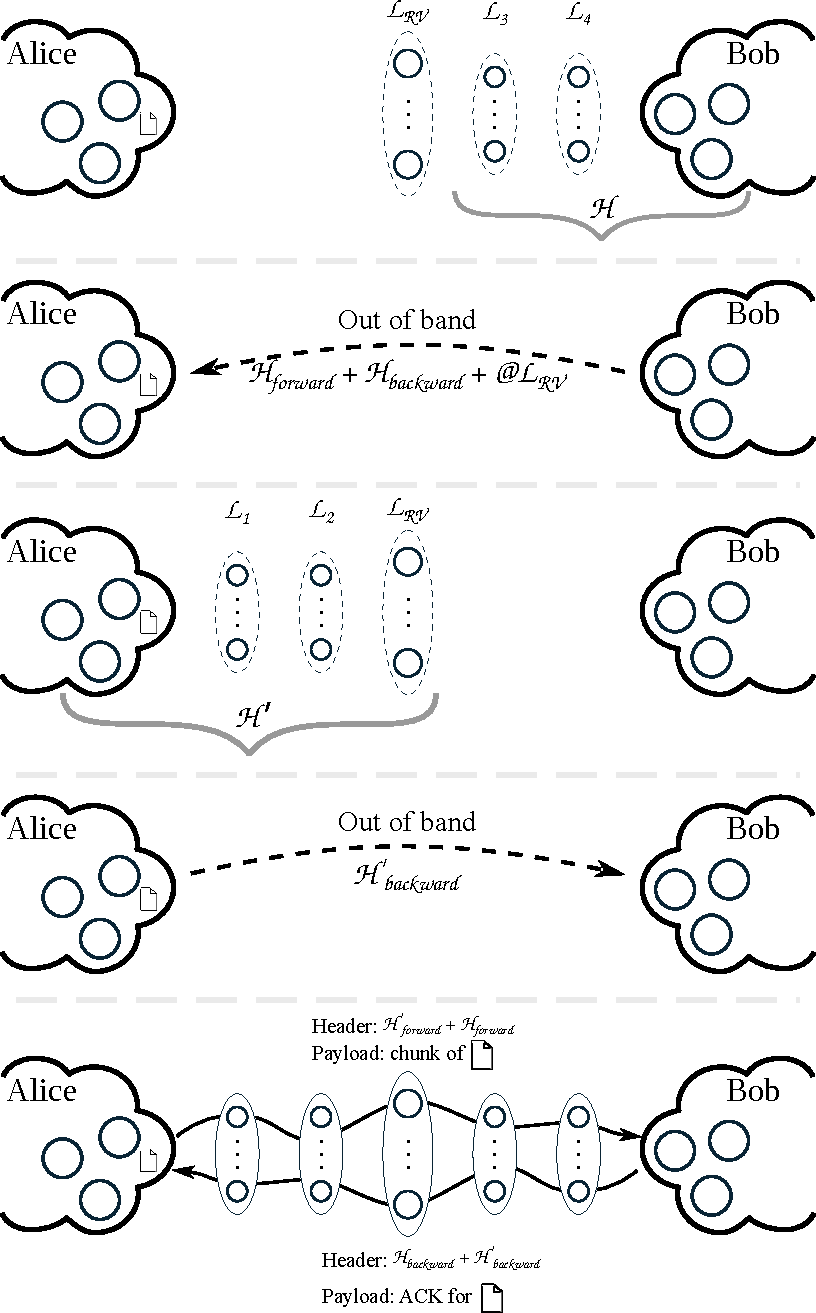
\includegraphics[width=\linewidth]{figures/file_exchange.pdf}
  \caption{\label{fig:file-exchange}A schematic of the creation and usage of PORs between Alice and Bob's e-squads.}
\end{figure}

\subsubsection{Building routes} 
\label{ssub:building_routes}

\commentAL{A symmetric key \datakey should be exchanged during this step, to encrypt the data}

When Alice wants to send a file $f$ to Bob, they first have to call the route building algorithm, and to exchange relevant information out of band (e.g. using mail, or their phones' bluetooth connection).
They create a route of $L$ layers, a configuration parameter that must be odd. We introduce $l=(L-1)/2$.

Bob (the receiver) initiates the route creation by calling the \Recv function displayed in figure~\ref{fig:route building algo}
He randomly chooses nodes to constitute a rendez-vous layer \LRV, and nodes to constitute $l$ layers from \LRV to his \squad. 
We come back on layer creation below.
He crafts a layered encrypted header (more details below) to \LRV (excluded) to his squad (included), that we will call \Hrecforward.
He also crafts his part of the header for the backward route, \Hrecbackward: it contains the route from Bob's \squad (excluded) to \LRV (included).

Bob then sends \Hrecforward and the descriptors of the \LRV nodes to Alice, by calling Alice's \Send function (also in figure~\ref{fig:route building algo}).
like Bob, Alice randomly picks nodes to constitutes $l$ layers from her \squad to \LRV.
She also builds two encrypted headers: \Hsendforward contains the route from her \squad (excluded) to \LRV (included), while \Hsendbackward contains the route from \LRV (excluded) to her \squad (included).
Alice now ha the full forward header \Hforward, as shown on line~\ref{hforward}
Alice finally sends \Hsendbackward back to Bob.

Back to \Recv function: Bob has the full backward header $\Hbackward$, as shown on line~\ref{hbackward}.


\paragraph*{Layer creation}
The function \CreateOnionLayer() iteratively adds random nodes (from the RPS's view \view) until the product $\prod_{d\in \mathcal{L}} (1 - p_d)$ falls below $\theta$.
$(1 - p_d)$ is the probability that a device $d$ will be offline; the product is the probability that all devices on layer $\mathcal{L}$ fall offline at the same time.


\begin{table}[t]
\resizebox{\columnwidth}{!}{
\begin{tabular}{lp{0.9\linewidth}}
\toprule
\multicolumn{2}{c}{\textbf{Parameters of the algorithm}} \\
\midrule
$\theta$ & Stopping criterion for the layers creation: maximum authorized  probability that all devices in a layer fail at once. \\
$L$      & Number of layers in a Predictive Onion Route. \\
$l = (L-1)/2$ & Number of layers (excluding $\LRV$) created by each end of the route. \\
\bottomrule
\end{tabular}
}
\label{tab:parameters}
\end{table}


\paragraph*{Header preparation} \commentAL{TODO}

\begin{figure}[t]
  %\framebox{\begin{minipage}{0.96\linewidth}
  \begin{algorithmic}[1]
    % \Require{%
    %   $D$ is the set of alternative recipient devices.
    % }
    \Function{\Recv}{sender}
      \State $\LRV \gets \CreateOnionLayer()$
      \State layers $\gets [\,]$
      \While{len(layers) $ < l$}
        \State layers.append(\CreateOnionLayer())
      \EndWhile
      \State $\Hrecforward \gets$ properly encrypted layers
      \State $\Hrecbackward \gets$ properly encrypted layers

      \Comment{Out-of-band exchange}
      \State $\Hsendbackward \gets$ sender.\Send(\Hrecforward, \LRV)

      \State $\Hbackward \gets \Hrecbackward \concat \Hsendbackward$ \label{hbackward}
      %\State $H_\rdv\gets \ExtendRoute[D\concat \top, L, \theta]$
      % \State \Return $H_\rdv$
      %   \Comment{Give to sender out-of-bound.}
    \EndFunction
  \end{algorithmic}
  %\end{minipage}}

  \vspace{0.3em}
  %\framebox{\begin{minipage}{0.96\linewidth}
  \begin{algorithmic}[1]
    % \Require{%
    %   $m$ is the message to be sent,
    %   $H_\rdv$ is the onion-route given by the recipient.
    % }
    \Function{\Send}{\Hrecforward, \LRV}
      \State layers $\gets [\,]$
      \While{len(layers) $ < l$}
        \State layers.append(\CreateOnionLayer())
      \EndWhile
      \State $\Hsendforward \gets$ properly encrypted layers
      \State $\Hsendbackward \gets$ properly encrypted layers
      \State $\Hforward \gets \Hsendforward \concat \Hrecforward$ \label{hforward}
      \State \Return \Hsendbackward


      \STATE $H\gets \ExtendRoute[H_\rdv, L, \theta]$
      \State $D\concat C_H\gets H_\rdv$
      \For{$d\in D$}
        \Comment{Uniformly randomly chosen}
        \If{$d\method \Fwd[C_H, m] \neq \bot$}
          \State \Return $\top$
        \EndIf
      \EndFor
      \State \Return $\bot$
    \EndFunction
  \end{algorithmic}
  %\end{minipage}}

  % \vspace{0.3em}
  % %\framebox{\begin{minipage}{0.96\linewidth}
  \begin{algorithmic}[1]
    \Require{%
      $H$ is a header of the form \(D\concat H'\) or \(D\concat \top\), where 
      \(D\) is a set of device addresses.
      $\pk_D$ is the public key of device set $D$.
      $L$ is the length of the route,
      $\theta$ is the threshold of probability of failure.%
    }
    \Function{\ExtendRoute}{$\mathcal{H}, l$}
      \If{$L\leq 0$}
        \State \Return $H$
      \EndIf
      \State $D\gets \CreateOnionLayer[\theta]$
      \State $H\gets D\concat \DeBEenc[\mpk, D, H]$
      \State \Return $\ExtendRoute[H, L-1, \theta]$
    \EndFunction
  \end{algorithmic}

  \vspace{0.3em}

  \begin{algorithmic}[1]
    \Function{\CreateOnionLayer}{\null}
      \State $(d, \pk_d, p_d)\gets \GetRandomPeer$
      \State $\mathcal{L}\gets \{(d, \pk_d, p_d)\}$
      \While{$\prod_{d\in \mathcal{L}} (1 - p_d) \geq \theta$}
        \State $(d, \pk_d, p_d)\gets \GetRandomPeer$
        \State $\mathcal{L}\gets \mathcal{L}\cup \{(d, \pk_d, p_d)\}$
      \EndWhile
      \State \Return $\mathcal{L}$
    \EndFunction
  \end{algorithmic}
  %\end{minipage}}
  \caption{\label{fig:route building algo}The route building algorithm}
\end{figure}


\subsubsection{Routing messages}
\label{ssub:routing_messages}


% Alice uses \(\Send\) at some
% later time to send the message to Bob using any of her devices from
% its \squad.% (See \cref{SPORSend}). 
% First, \(\Send\) extends the route
% \(H_\rdv\) with some hops of Alice's choosing (uniformly randomly
% chosen). Second, \(\Send\) extracts from the onion the first
% layer, which contained the overall
% possible rendez-vous points $D$ previously selected by the recipient (i.e. Bob).
% One device from $D$ is randomly chosen, and the \(\Fwd\)
% sub-function is called as long as the message forwarding to one node of
% the next layer is not successful.% (See \cref{SPORFwd}). 
% Along the path, each node decrypts
% in sequence the different layer with the current node’s private key. 
% The end of the route is reached when special value \(H_\rdv = \top\) is
% encountered. Consequently the ciphered message \(c_m\) is then stored
% in the disk of the local node through the \(\Store\) sub function.%(\cref{SPORRecv}).

\begin{figure}[t]
  %\framebox{\begin{minipage}{0.96\linewidth}
  \begin{algorithmic}[1]
    %\Require{$\pk, \sk$ is the public--private key-pair of the node.}
    \Function{\Fwd}{$C_H, m$}
      \State $H\gets \DeBEdec[\mpk, \sk, C_H]$
      \If{$H = \bot$}
        \State \Return $\bot$
      \EndIf
      \State $\{d_i\}\concat C_H'\gets H$
      \If{$C_H' = \top$}
        \State \Return $\Store[m]$
      \EndIf
      \For{$d\in \{d_i\}$}
        \Comment{Uniformly randomly chosen}
        \If{$d\method \Fwd[C_H', m] \neq \bot$}
          \State \Return $\top$
        \EndIf
      \EndFor
      \State \Return $\bot$
    \EndFunction
  \end{algorithmic}

  \begin{algorithmic}[1]
    \Function{\Store}{$m$}
      \State $m\gets \DeBEdec[\mpk, \sk, c_m]$
      \If{$m = \bot$}
        \State \Return $\bot$
      \EndIf
      \State Store $m$ to disk.
      \State \Return $\top$
    \EndFunction
  \end{algorithmic}
  %\end{minipage}}
  \caption{\label{SPORFwd}%
    The \(\Fwd\) algorithm forwards \(m\) down the route \(H\), obtained 
    by decrypting \(C_H\) with the node's associated private key.
    The special value \(H = \top\) indicated the end of the route, thus \(c_m\) 
    is intended for the local node and \(c_m\) is instead sent to disk using 
    \(\Store\).% (\cref{SPORRecv}).%
  }
\end{figure}

\subsubsection{Exchanging a file} % (fold)
\label{ssub:exchanging_a_file}

% subsubsection exchanging_a_file (end)
\newcommand{\messagesize}{\ensuremath{s_m}}
\newcommand{\filesize}{\ensuremath{s_f}}
\newcommand{\headersize}{\ensuremath{s_{\mathcal{H}}}}

Once Alice get the \Hforward, she can start sending her file $f$ to Bob. 
To do so, she chunks it to pieces, and iteratively send the chunks to Bob, that replies with an acknowledgment (ACK) for that chunk.
Once all chunks have been acknowledged, Alice sends an empty message to Bob, signifying transfer termination.

To prevent \name from message size analysis attacks, the messages have a fixed size \messagesize.
As shown in the previous section~\ref{ssub:building_routes}, headers have a variable size \headersize per route (but \Hforward remains constant once the POR is established).
For this reason, file chunks have a fixed size per session: $\filesize = \messagesize - \headersize$.

A message payload is composed of the following information:

\begin{itemize}
  \item An identifier for the file;
  \item The chunk ID, that identifies its position in $f$;
  \item The file chunk;
  \item An error correction code (e.g. a SHA-1 hash of the chunk, à la BitTorrent\cite{bt_bep3}).
\end{itemize}

Payloads are encoded using \datakey that was shared between Alice and Bob during route creation \commentAL{Not done}.


% We are interested in transferring large files.
% Every device \(d\in D\) in the global device swarm is only periodically online.
% We will thus divide the data to send into \(n\) smaller chunks (similar to 
% BitTorrent~\cite{BitTorrent}).
% The idea is to choose \(n\) such that each chunk will be small enough to be 
% successfully relayed by a device before it goes offline again.
% The chunk size is empirically determined in \cref{Performance}.
% \commentDaniel{Adrien, is that true?}

% As stated above, Alice and Bob exchange some limited data out-of-bound using 
% their smartphones.
% The information they will exchange is the following:
% \begin{enumerate}
%   \item Bob creates an onion route header, \(H_\rdv\), by running 
%     \([\Recv]\) %(\cref{SPORRecv}) 
%     and gives it to Alice.
%   \item Alice gives Bob number of file chunks, \(n\), and the size of the file 
%     chunks.
%   \item They agree on a file-specific key \(k\) for some (authenticated) 
%     encryption scheme \(\Enc*\).
% \end{enumerate}
% Then Alice encrypts the file \(f\) and receives the ciphertext \(c_f\gets 
%   \Enc*[Enc](k, f)\).
% She then divides \(c_f\) into \(n\) chunks, \(c_f^{(1)}, \dotsc, c_f^{(n)}\), 
% and runs \(\Send(H_\rdv, c_f^{(i)})\) for all \(1\leq i\leq n\) in 
% parallel.
% \commentDaniel{Or shall we do it sequentially?}










% For instance, if Alice wants to send a message \(m\) to Bob, they are both going to perform a part of the building algorithm.
% Bob uses the \([\Recv]\) function (See \cref{SPORRecv}) to create a probabilistic onion route $\mathcal{H_B}$ from
%  a rendez-vous (RV) layer $\mathcal{L_{RV}}$ to its own devices from its \squad---all the hops on the route are 
% chosen by Bob uniformly at random from the Global Overlay.
%  \(\SPOR[\Recv]\)
% returns $\mathcal{H_B}$ and  that Bob gives to Alice using an
% out-of-band channel, \eg using one device of its \squad.
% PORs have \(L\) layers, and for each layer the number of
% alternatives nodes depends of a failure threshold \(\theta\). 
% As long as \(\theta\) is not exceeded, alternatives nodes are added in
% \(H_\rdv\) as depicted in \cref{ExtendRoute}. Thus the probability of
% failure for the extension is \(1 - (1 - \theta)^L\).

% Once Alice get the \(H_\rdv\), Alice uses \(\SPOR[\Send]\) at some
% later time to send the message to Bob using any of her devices from
% its \squad (See \cref{SPORSend}). First, \(\SPOR[\Send]\) extends the route
% \(H_\rdv\) with some hops of Alice's choosing (uniformly randomly
% chosen). Second, \(\SPOR[\Send]\) extracts from the onion the first
% layer, which contained the overall
% possible rendez-vous points $D$ previously selected by the recipient (i.e. Bob).
% One device from $D$ is randomly chosen, and the \(\SPOR[\Fwd]\)
% sub-function is called as long as the message forwarding to one node of
% the next layer is not successful (See \cref{SPORFwd}). Along the path, each node decrypts
% in sequence the different layer with the current node’s private key. 
% The end of the route is reached when special value \(H_\rdv = \top\) is
% encountered. Consequently the ciphered message \(c_m\) is then stored
% in the disk of the local node through the \(\Store\) sub function 
% (\cref{SPORRecv}).



%The special value \(H = \top\) indicated the end of the route, thus \(c_m\) 
%    is intended for the local node and \(c_m\) is instead sent to disk using 
%    \(\Store\) (\cref{SPORRecv}).% 


%The SPOR.Forward algorithm forwards m down the route H, obtained by
%decrypting CH with the node’s associated private key. The special
%value H = ⊤ indicated the end of the route, thus cm is intended for
%the local node and cm is instead sent to disk using Store

%extends the route \(H_\rdv\) (using 
 %   \(\ExtendRoute\), \cref{ExtendRoute}) and sends the message \(m\) down the 
  %  extended route using the \(\SPOR[\Fwd]\) algorithm (\cref{SPORFwd}).
   % The first node of \(H_\rdv\) is the rendez-vous point selected by the 
    %recipient.

%It creates a probabilistic onion-route from a rendez-vous point to its own 
%    devices and returns the route to the sender.
 





